\section{Acoustic Bump}

% Describe test case
% - open-closed tube
% - A J_1 bump in the middle (easy to calculate approximately under linearity assumption) which travels to the left in the DNS region to begin with
% - Enforce ADCBC inflows and outflows in a thin DNS region to approximate the 1D acoustic problem as with a 2D domain
% - The full reacting Navier-Stokes equations are solved in the DNS region as a precursor to a flame being in the DNS region. The boundary conditions also work almost identically in this case under the viscous, inert, isothermal equations which are also implemented in the SUNSET code, but are not used here.
% - For thin regions like this the averaging along the boundary makes sense, but as the DNS domain widens, it seems reasonable that this averaging would result in more and more inaccuracy (and difficulty due to instability...), so the similar method where queues are used for each boundary node should instead be used in wider domains. For all the cases in this report, the averaging procedure is used and we find good results regardless.


% Acoustic region postprocessing
% - theoretically how could this work in the ADCBC framework?
% - log stored queue values at specific non-dimensional times which are interpreted as time series of characteristic waves leaving the inflow or outflow DNS boundary
% - According to the same linear approximation made on acoustic waves under the ADCBC formulation, we can reinterpret these time series as spatial information: the longer ago the acoustic exited the domain, the farther into the acoustic domain (or back towards the DNS domain) they will be
% - This only requires the queue information, sound speed and u to calculate upstream and downstream L_1 and L_5 values, then to calculate upstream and downstream u and p values we integrate L_1 and L_5 starting from the DNS inflow or outflow u and p alongside rho (for u?)


% Acoustic bump results
% - Show result of a Gaussian bump leaving the domain and reentering after 1 bounce, 2 bounce (each boundary) and 100 bounces

\begin{figure}[t]
\centering
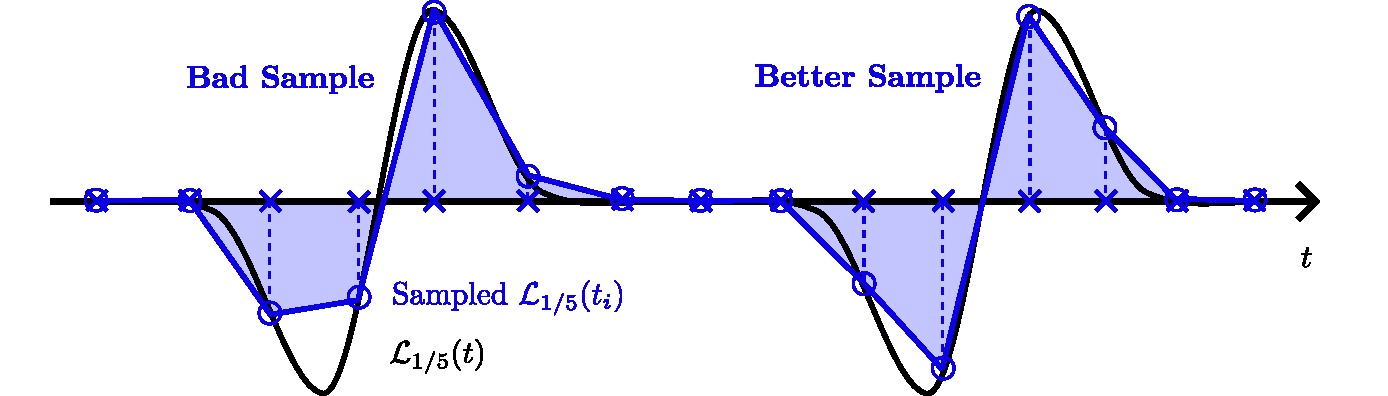
\includegraphics[scale=0.65]{assets/imgs/wave-sampling-comparison.pdf}
\caption{SAMPLING}
\label{fig:wave-sampling}
\end{figure}

% Now is a good time to bring up the sampling error
% - \fig{fig:wave-sampling} shows a representative analytic L_{1/5} field for two acoustic bumps (which is roughly the derivative of the Gaussian). Despite the same linear interpolation and sample period being used, the sampled $L$ values on the left are much worse than on the right. The same could be true for any number of samples at a constant interpolation order and sample period, where the change in phase of the sampling with the wave will always cause some inaccuracy in the integrated acoustic field. This inaccuracy results in a change to the shape of the Gaussian, e.g. a skew to one side, which feeds back into this issue such that the waves eventually fully break down
% - For the acoustic bump in this small domain this seems to happen relatively quickly because the associated acoustic frequencies of this system are higher. But, if the bump remains the same size and the tube is made longer, less bounces happen and the sampling error grows slower
% - Furthermore, there is the added effect that natural wavenumbers of these longer tubes will be lower, meaning that individual waves can be sampled better. This leads to an asymptotic behaviour of O(l^2) for values of error productions which are small (DO SOME MATHS?).

% Different interpolation orders:
% - Constant interpolation maintains the quality of acoustic bump surprisingly well, whilst the non-constant interpolation seems to introduce some small error on every reentry of the acoustic bump
% - simplest explanation (which isn't just a fault implementation) seems like the act of 






\section{Acoustic Standing Wave}

% Describe test case
% - An acoustic standing wave. Calculated differently to the acoustic bump by 


% bring up instability issue here not before (because it's a practical issue)!

% We can also see the sampling instability in the standing wave results as a q-wave \cite{poinsot2001TheoreticalNumericalCombustion} which is largest at maximum values of L???
% Show image/s
% Easiest to see when instability is not present



\section{Thermoacoustically Unstable Flame}


\begin{figure}[t]
\centering
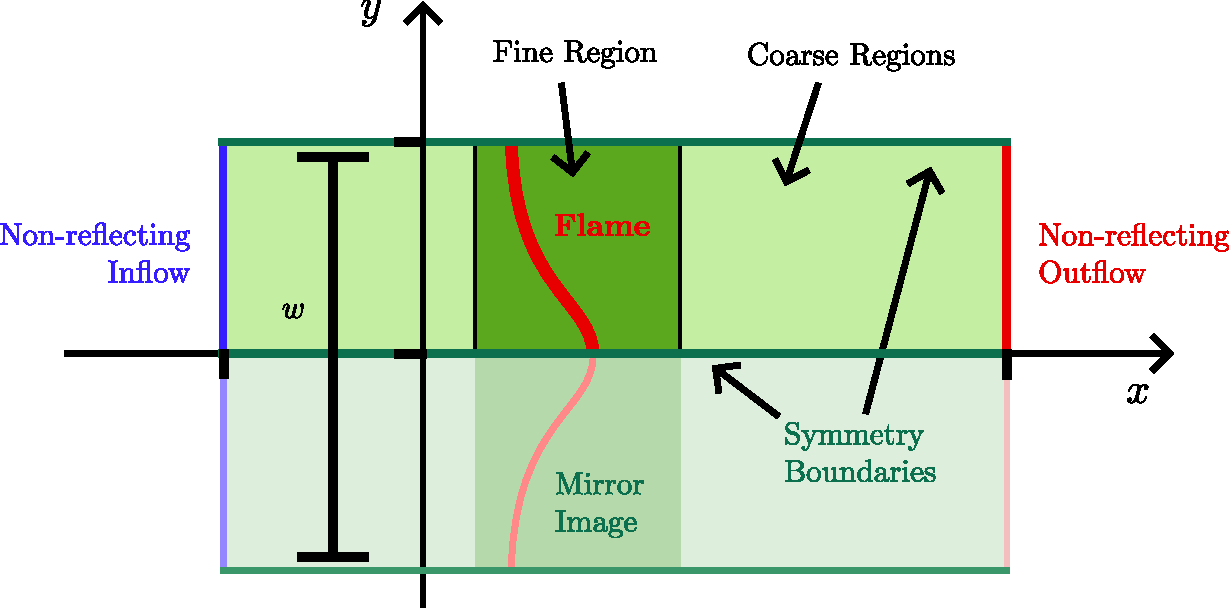
\includegraphics[scale=0.65]{assets/imgs/DNS-computational-domain.pdf}
\caption{DNS COMPUTATIONAL DOMAIN}
\label{fig:DNS-domain}
\end{figure}


% It may seem like a large jump to go from inert, essentially isothermal acoustics to fully reacting flame-acoustic interactions, but the sunset code is designed with flame simulations in mind, so the simulations are 'easy' to perform having already implemented ADCBC.
% (Maybe there are better intermediate test cases? D-TDIBC don't seem to need them)





\subsection{Prediction from Eigenmodes}


\begin{figure}[t]
\centering
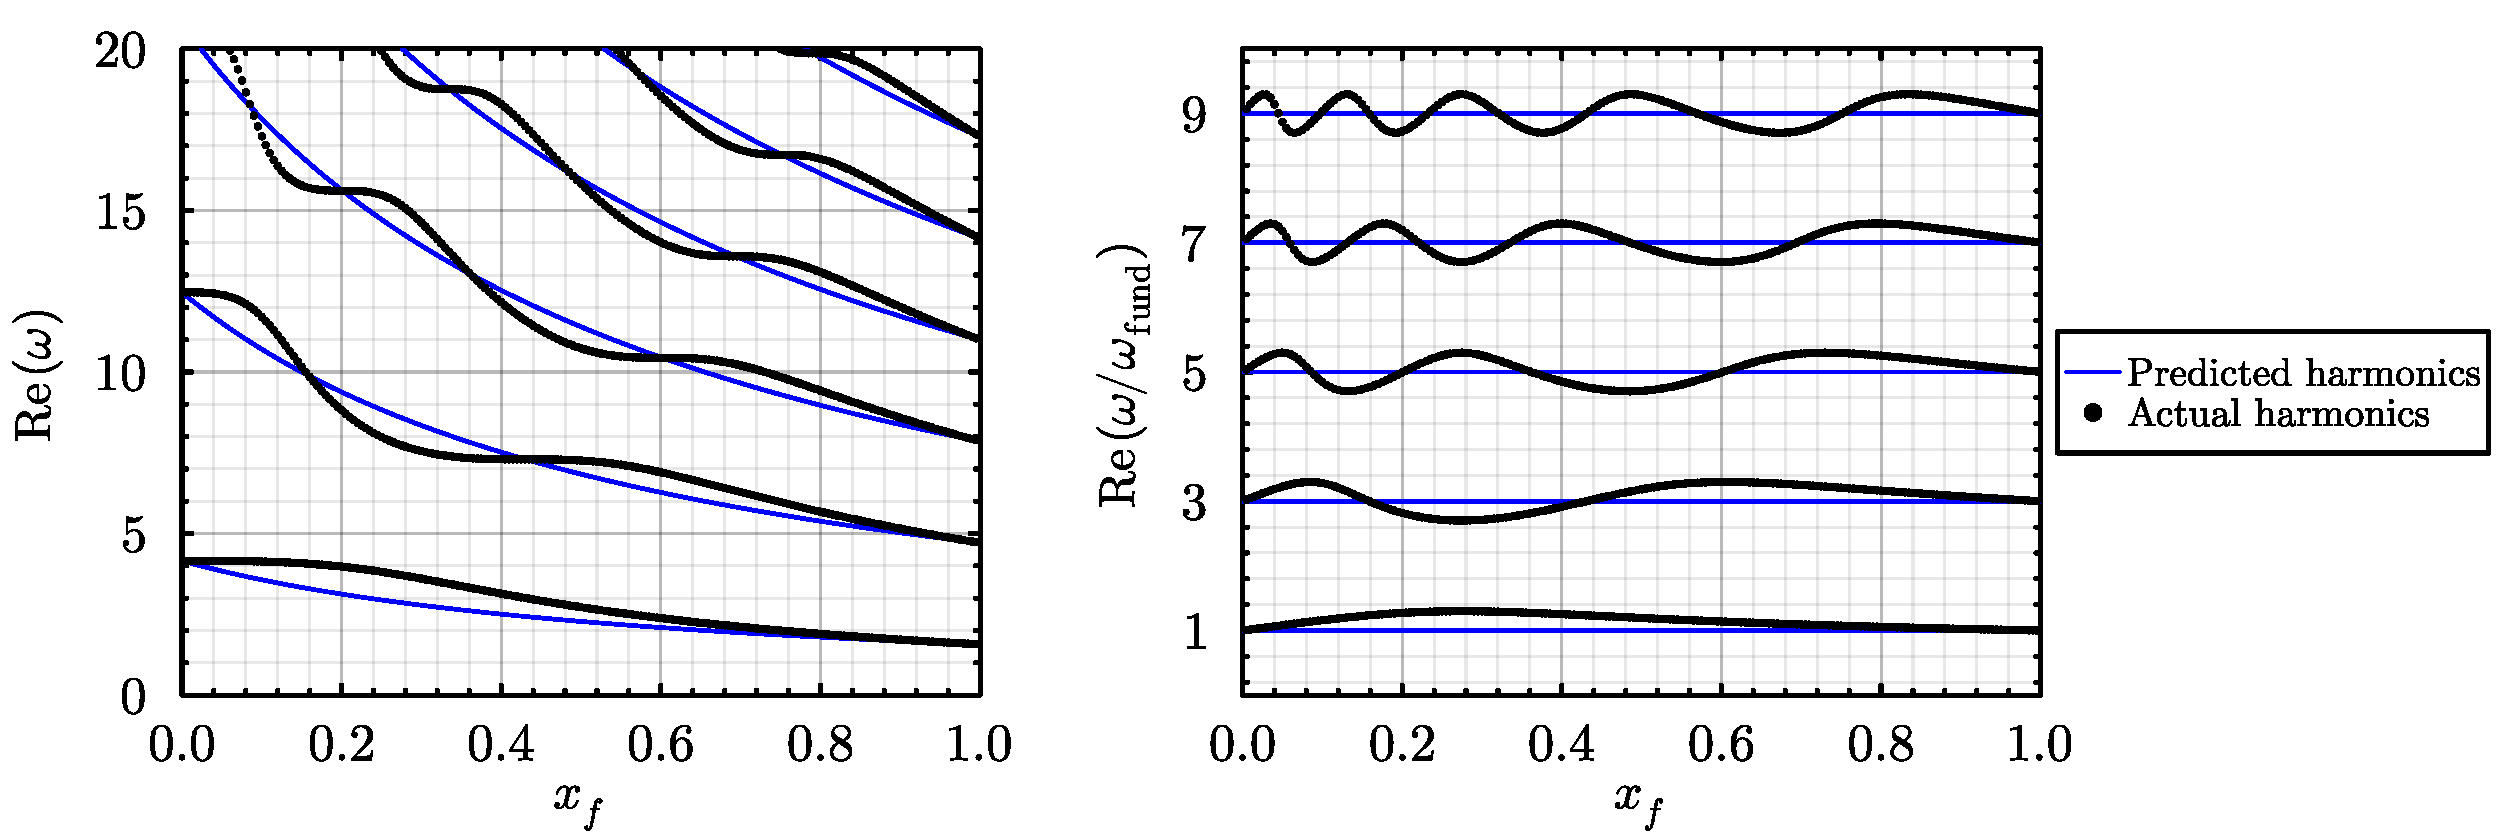
\includegraphics[scale=0.35]{assets/graphs/r=7_harmonics_both.pdf}
\caption{$r = 7$, LEFT: , RIGHT: divided by }
\label{fig:flame-harmonics}
\end{figure}

\begin{figure}[t]
\centering
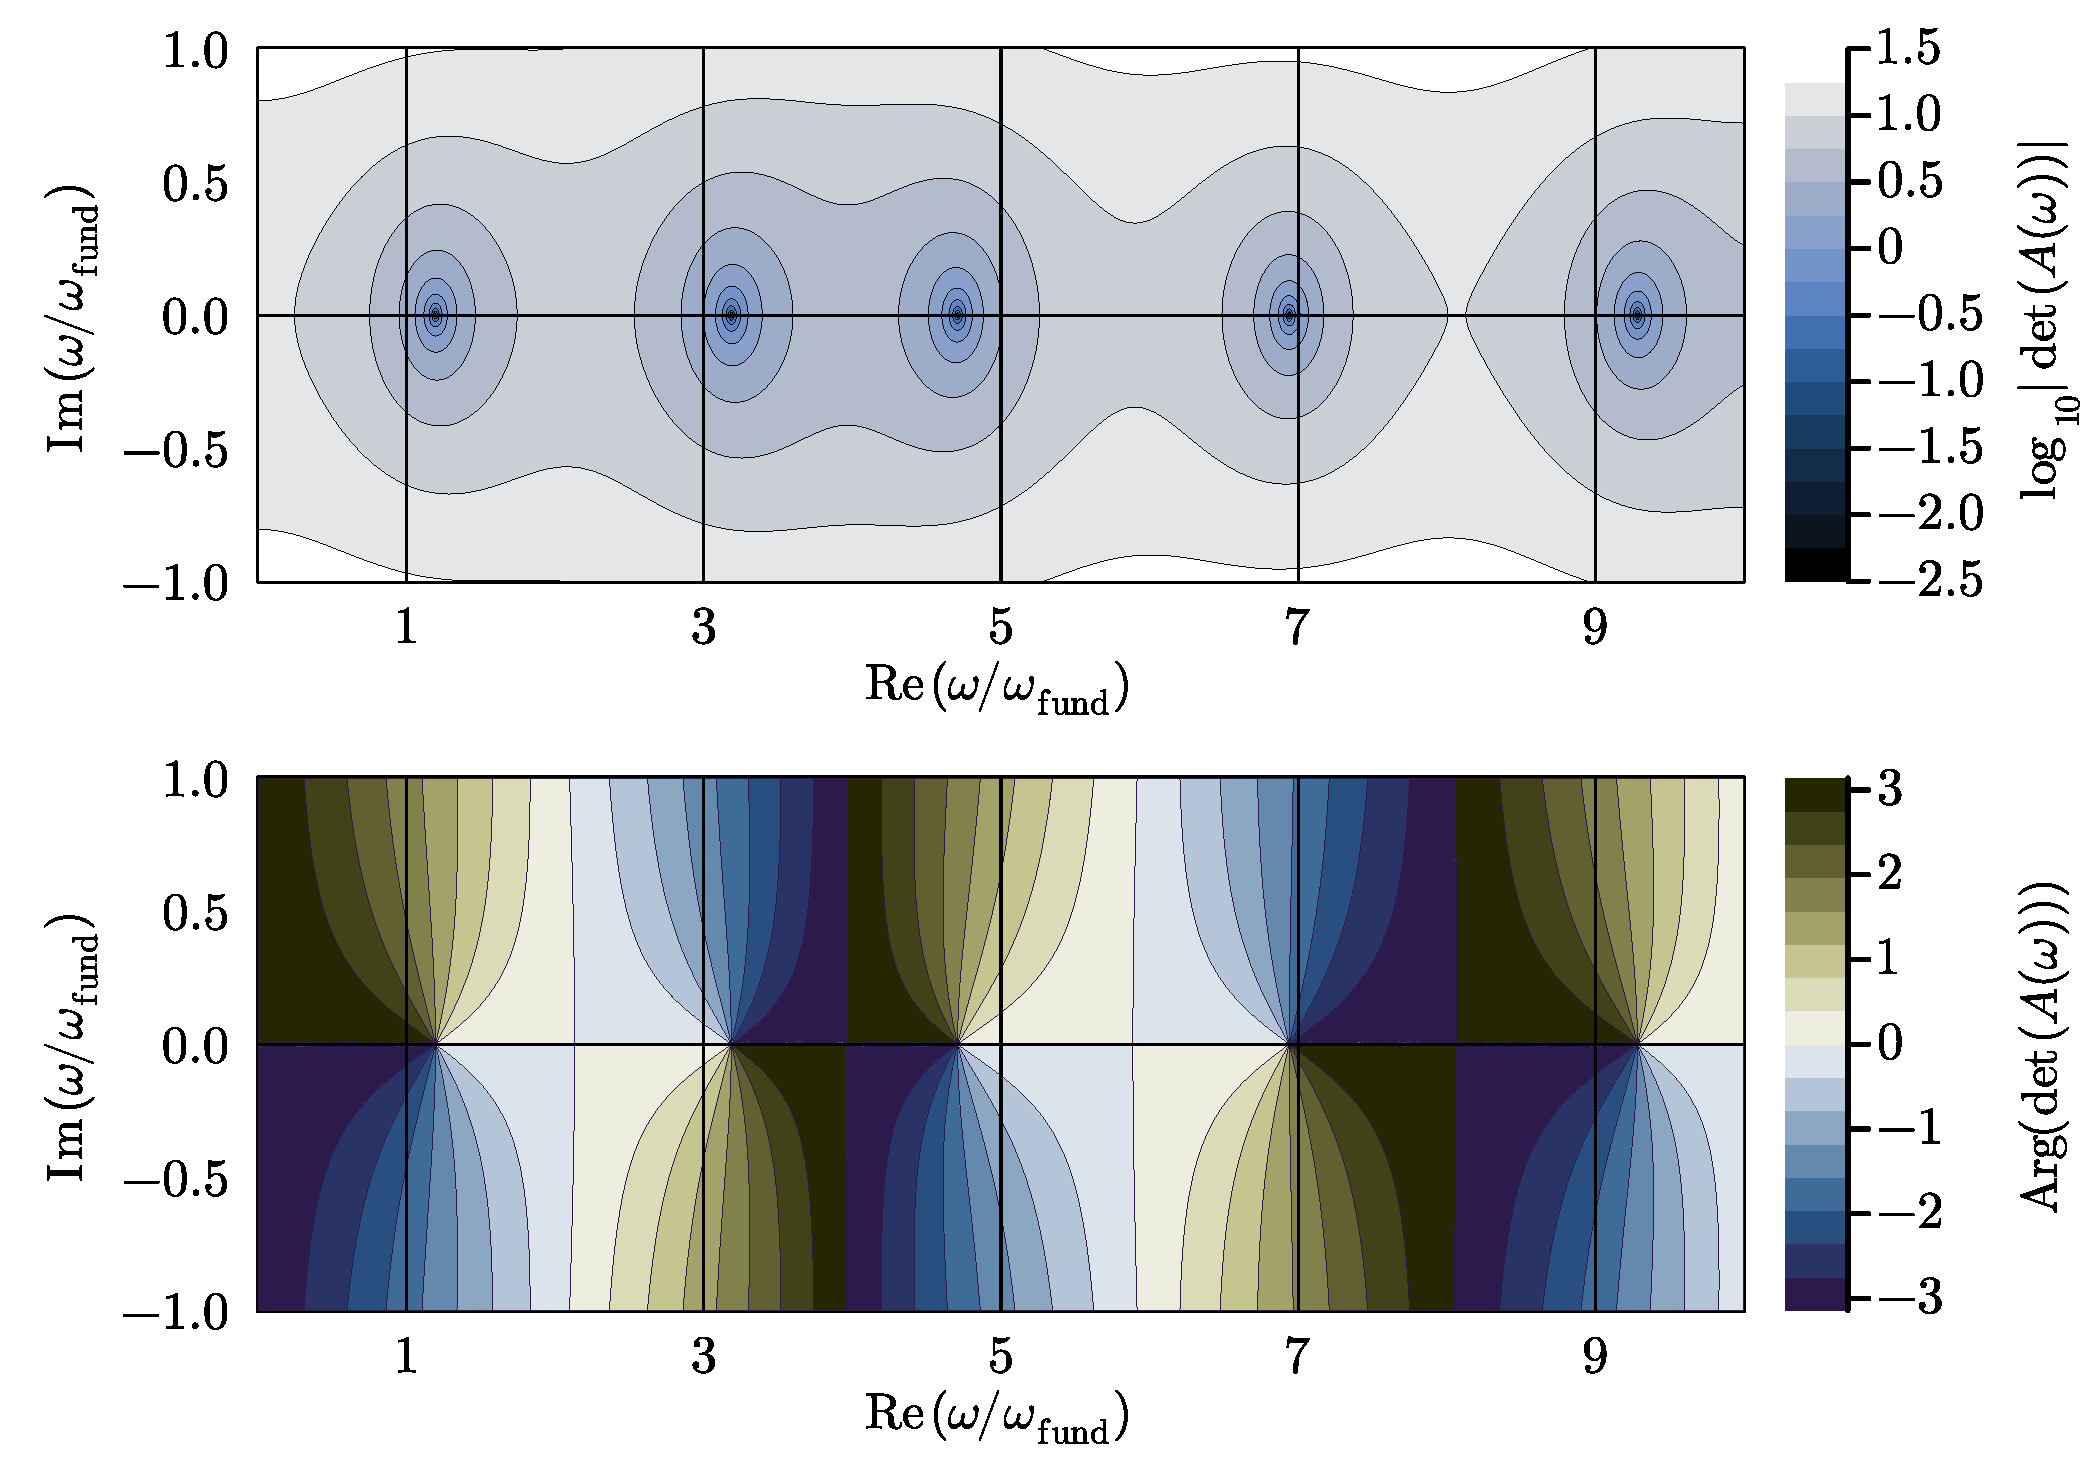
\includegraphics[scale=0.35]{assets/graphs/r=7_xf=05_complex_harmonics.pdf}
\caption{$r = 7, x_f = 0.5$, CAPTION}
\label{fig:flame-harmonics-complex}
\end{figure}




\subsection{DNS Results}


% stats data fft postprocessing/windowing
% spectrogram results
% frequencies
% mode structures!



\begin{figure}[t]
\centering
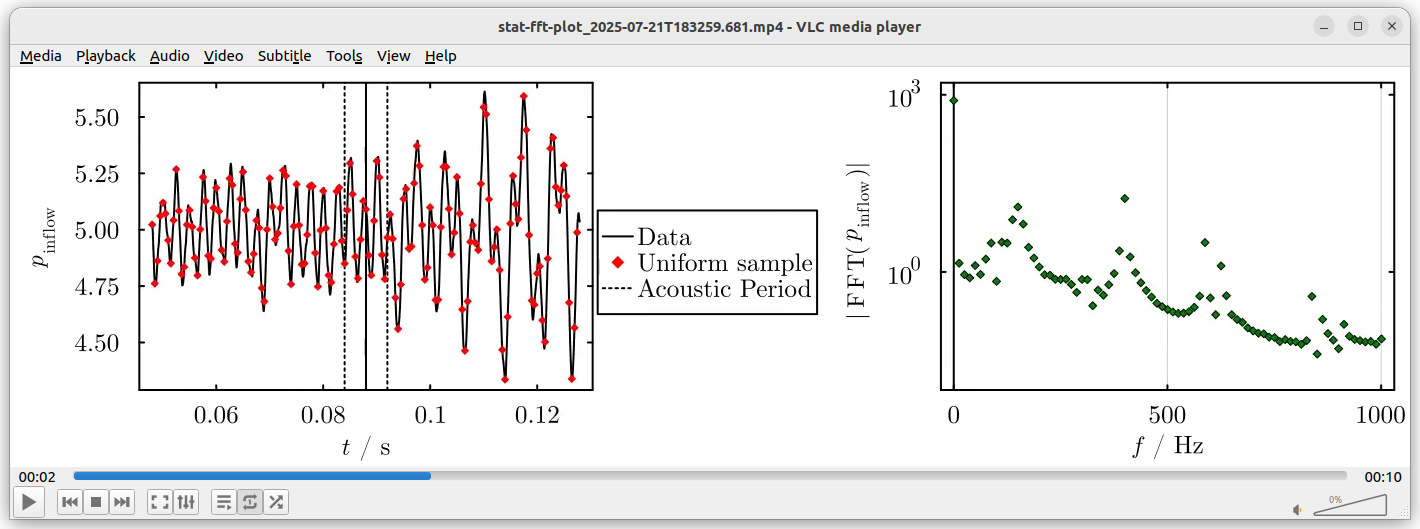
\includegraphics[scale=0.35]{assets/graphs/fft-windowing.png}
\caption{[PLACEHOLDER IMG] FFT WINDOWING}
\label{fig:windowing}
\end{figure}

\begin{figure}[t]
\centering
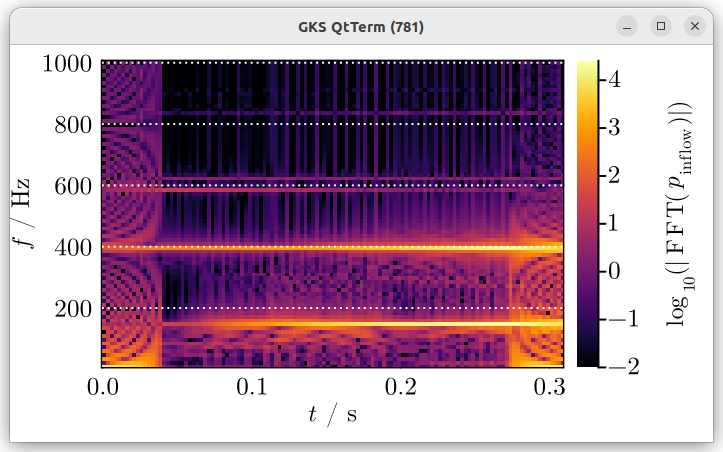
\includegraphics[scale=0.35]{assets/graphs/spectrogram.png}
\caption{[PLACEHOLDER IMG] SPECTROGRAM}
\label{fig:spectrogram}
\end{figure}

\begin{figure}[t]
\centering
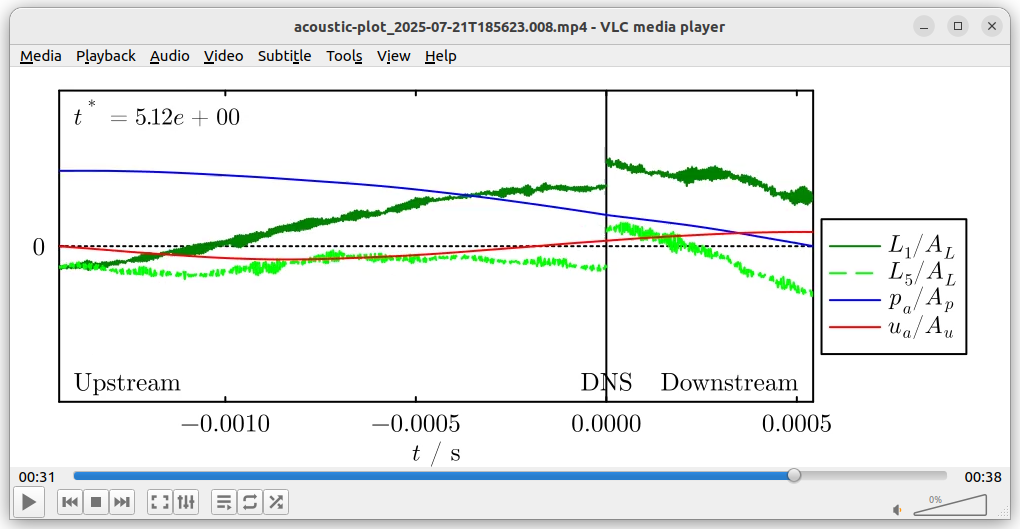
\includegraphics[scale=0.35]{assets/graphs/pp-tones.png}
\caption{[PLACEHOLDER IMG] POST-PROCESSED 1/4 AND 3/4 WAVE EVIDENCE}
\label{fig:pp-tones}
\end{figure}


